\documentclass[tikz, border=10pt]{standalone}
\usepackage{tikz}
\usetikzlibrary{positioning, arrows.meta, backgrounds}

\tikzstyle{n} = [circle, draw, minimum size=0.8cm]

\begin{document}
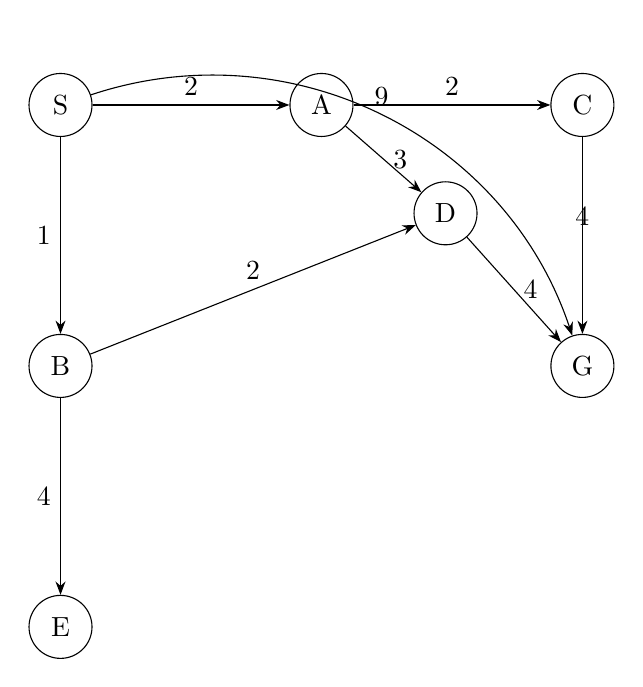
\begin{tikzpicture}[>=Stealth, node distance=2.5cm and 2.5cm]

    \node[n] (S) {S};
    \node[n, right=of S] (A) {A};
    \node[n, below=of S] (B) {B};
    \node[n, right=of A] (C) {C};
    \node[n, below=of C] (G) {G};
    \node[n, below right=0.8cm and 1cm of A] (D) {D};
    \node[n, below=of B] (E) {E};

    \path[->]
        (S) edge node[above] {2} (A)
        (S) edge node[left] {1} (B)
        (A) edge node[above] {2} (C)
        (C) edge node[above] {4} (G)
        (A) edge node[right] {3} (D)
        (B) edge node[above] {2} (D)
        (B) edge node[left] {4} (E)
        (D) edge node[right] {4} (G)
        (S) edge [bend left=45] node[above] {9} (G)
    ;

\end{tikzpicture}
\end{document}